\section{Experimental results}

We tested the methodology outlined in section~\ref{sec:method} on the
publicly available git repositories for two popular open source
projects, the ANTLR parser generator and the Clojure language implementation.
Both are implemented in Java, and one (ANTLR) is composed of a mixture of
hand-written and automatically generated code.  

\subsection{Threshold sensitivity}

The first experiment that we performed was to investigate the effect of
similarity threshold to the number of groups identified, as well as the degree
of generality present in the tree that results from all members of each group
being anti-unified together. Our prediction was that at the lowest threshold
(0.0), when all trees are considered to be similar, their anti-unification
will yield the most general pattern.  This is what was observed, in which the
anti-unification result is a tree composed of a single metavariable node.
Similarly, at the highest threshold (1.0), the only groupings that will be
present will be single tree sets, or sets containing identical trees for
instances of identical changes that occurred in different places.  This is
precicely what we observed, with the anti-unified trees containing no meta-
variables since anti-unification of a set of identical elements is the element
itself.  We show the number of groups (broken down by type: code addition,
code deletion, or code mutation) as a function of threshold in
Figure~\ref{fig:thresholdplot}.

As we can see, as the threshold increases, we see more groupings of changes
due to changes that were considered similar under a lower threshold being
considered dissimilar under the more restrictive threshold.  For example, at
$t=0.15$, a single pattern for for-loops is identified:

\begin{verbatim}
for ([]=[];[]<[];[]) {
    []
}
\end{verbatim}

As the threshold is increased to $t=0.25$, in addition to generic for-loops, a
cohort of changes are identified to a more specific instance of the for-loop where
the loop counter is initialized to zero:

\begin{verbatim}
for ([]=0;[]<[];[]) {
    []
}
\end{verbatim}

Increasing to $t=0.35$, the pattern for the conditional becomes more specific
and we see what appears to be a template for using the field of an object
(e.g., {\tt args.length}) as the loop termination criterion:

\begin{verbatim}
for ([]=0;[]<[].[];[]) {
    []
}
\end{verbatim}

Similar templates emerge for code patterns such as method invocations, printing
the concatenation of two strings, and other common activities.  

\subsection{Group sizes}

\subsection{Pattern identification}

Using a portion of the Clojure history, we computed the number of similar trees
at each threshold. See figure~\ref{fig:clojure-number-of-modifications} to see
the number of changes by time as a function of the threshold. We looked at
thresholds from 0 to 1 with an increment size of 0.01.

\begin{figure}
\begin{center}
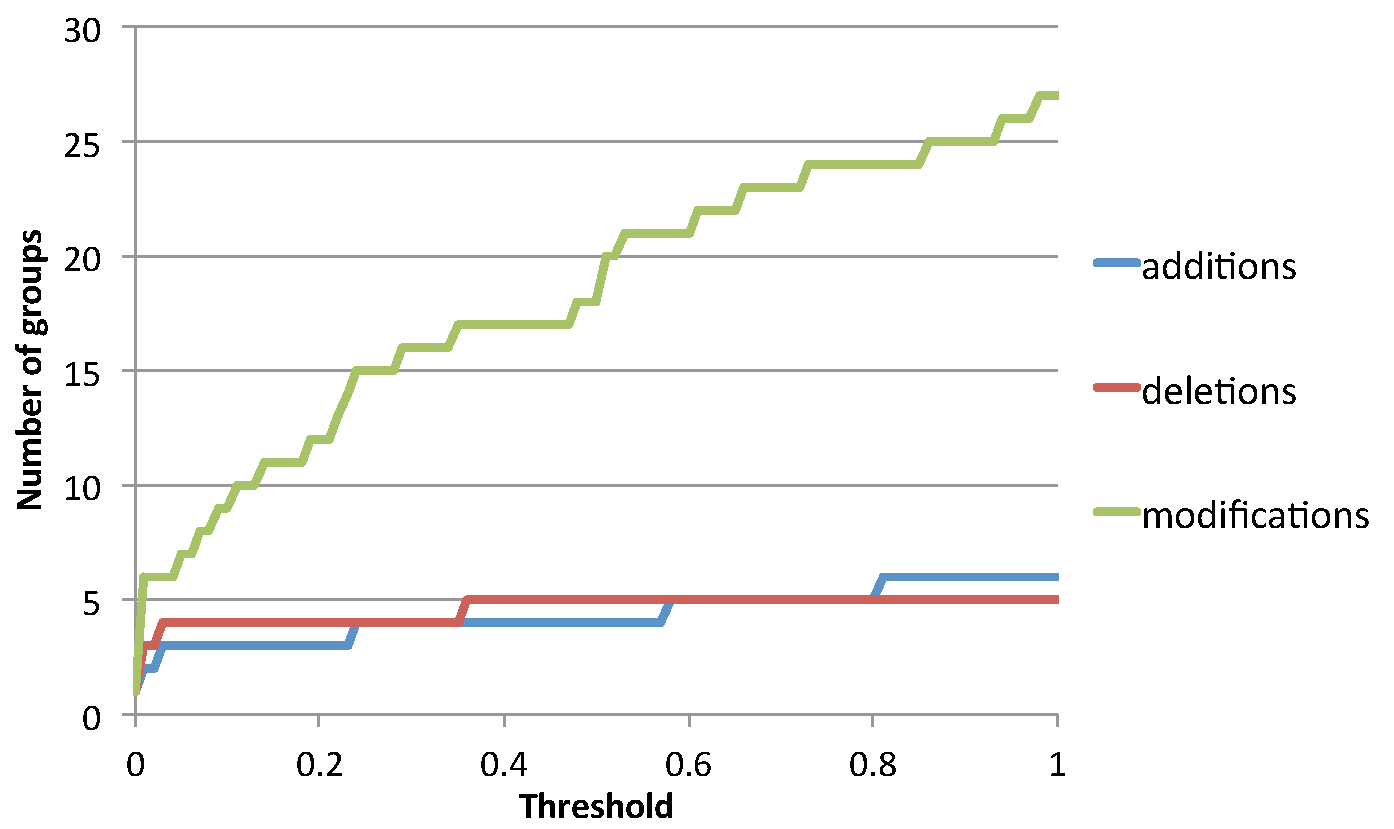
\includegraphics[width=0.44\textwidth]{figures/clojure-number-of-modifications.pdf}
\caption{Number of additions, deletions, and modifications by threshold for the Clojure source}
\label{fig:clojure-number-of-modifications}
\end{center}
\end{figure}

\begin{figure}
\begin{center}
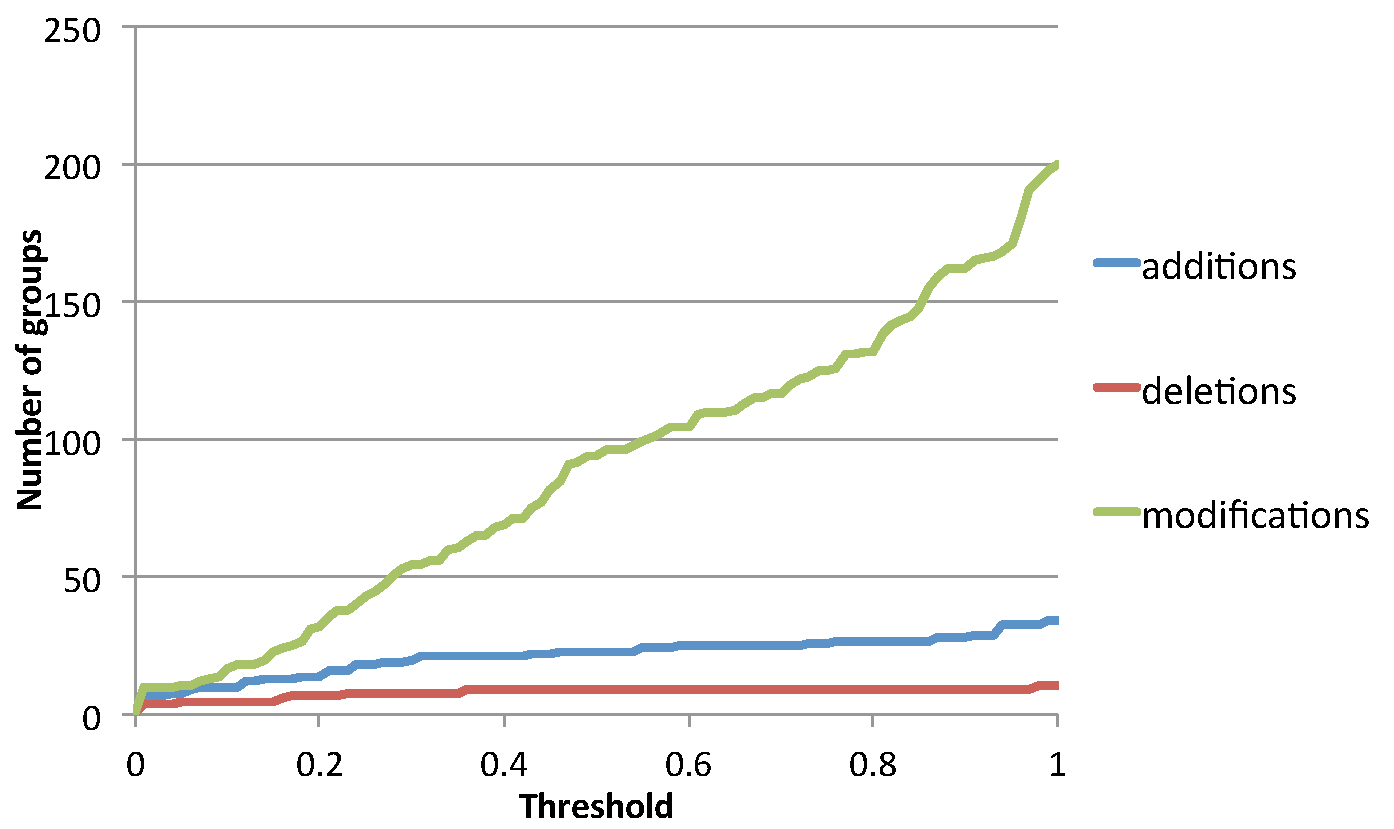
\includegraphics[width=0.44\textwidth]{figures/antlr-number-of-modifications.pdf}
\caption{Number of additions, deletions, and modifications by threshold for the Antlr source}
\label{fig:antlr-number-of-modifications}
\end{center}
\end{figure}

Looking at just the number of deletions, we examined the point where the number
of deletions goes from 4 to 5 as the threshold changes from 0.35 to 0.36.

The following code, presented in a standard diff format, shows a loop and the
lines that were removed. This example comes from a file named {\tt
PersistentArrayMap.java }.

\subsubsection{Removed code}
\begin{verbatim}
 public Object kvreduce(IFn f, Object init){
     for(int i=0;i < array.length;i+=2){
         init = f.invoke(init, array[i], array[i+1]);
-           if(RT.isReduced(init))
-                   return ((IDeref)init).deref();
         }
     return init;
 }
\end{verbatim}

Given the low threshold, this deletion was considered to be similar to the
following deletions. This example comes from {\tt PersistentHashMap.java}.
Note: Our parser ignores whitespace and gives the same AST for \verb|if (exp) { stmt; }|
and \verb|if (exp) stmt;|. In the diff below, we have prefixed the
lines that were considered to actually be different by our tool with ``>''
characters.

\begin{verbatim}
     public Object kvreduce(IFn f, Object init){
-        for(INode node : array){
-            if(node != null){
+        for(INode node : array)
+            {
+            if(node != null)
                 init = node.kvreduce(f,init);
>-                   if(RT.isReduced(init))
>-                           return ((IDeref)init).deref();
-                   }
-               }
+            }
         return init;
     }
\end{verbatim}

In both cases, our tool identified for-loops where the the same lines are
removed. In fact, the code for both of these is very similar perhaps owing to
Java's HashMap and ArrayMap classes being very similar in terms of interface.
Furthermore, it did this at the statement level, eg., we did not need to
consider the similarities of the file names or the method names.

%% Doctored version
%%\begin{verbatim}
%% public Object kvreduce(IFn f, Object init){
%%     for(INode node : array){
%%         if(node != null)
%%-        {
%%             init = node.kvreduce(f,init);
%%-            if(RT.isReduced(init))
%%-                    return ((IDeref)init).deref();
%%-        }
%%     }
%%     return init;
%% }
%%\end{verbatim}


\subsection{Interpretation of results}

